
% how to compile: platex xxx.tex ; dvipdfmx xxx.dvi

\documentclass[a4paper]{jarticle}


%--余白の設定
\setlength{\topmargin}{20mm}
\addtolength{\topmargin}{-1in}
\setlength{\oddsidemargin}{20mm}
\addtolength{\oddsidemargin}{-1in}
\setlength{\evensidemargin}{15mm}
\addtolength{\evensidemargin}{-1in}
\setlength{\textwidth}{170mm}
\setlength{\textheight}{254mm}
\setlength{\headsep}{0mm}
\setlength{\headheight}{0mm}
\setlength{\topskip}{0mm}

%--ハイバーリンクを可能にするパッケージ
\usepackage[dvipdfmx,%
 bookmarks=true,%
 bookmarksnumbered=true,%
 colorlinks=true,%
 setpagesize=false,%
 pdftitle={mcat},%
 pdfauthor={BMRC},%
 pdfkeywords={TeX; dvipdfmx; hyperref; color;}]{hyperref}

\usepackage{graphicx}
\usepackage{tabularx}

\begin{document}

\setlength{\baselineskip}{4mm}

\section*{kago\_sequence.rb 系列パターンの列挙}
アイテム系列データから頻出系列パターンを列挙する。
アイテム系列データとは、順序付けられたアイテム列の集合であり、
アイテム系列データに多く「出現」する部分系列のことである。
「出現」の定義は後述する。
列挙のコアアルゴリズムにはLCMseq(LCM algorithm for enumerating all frequently appearing sequences)を用いている\cite{UnoWeb}。
本コマンドは以下のような特徴を持つ。
\begin{itemize}
 \item 他のパターンに含まれないパターン(極大パターン)を列挙することができる。
%\item 同一の出現件数における極大パターン(飽和パターン)を列挙することができる。
 \item あるクラスに特徴的なパターン(顕在系列パターン)を列挙することができる。
 \item アイテムの分類階層(taxonomy)を用いることができる。
 \item gap長とwindow幅の制約条件(上限値)を与えることができる。
 \item gap長とwindow幅の制約条件(上限値)を時間制約として与えることも可能。
 \item アイテム集合のシーケン(同じ時刻に異なる複数のアイテム)は扱うことはできない。
\end{itemize}

表\ref{tbl:seqDB}に、本コマンドが扱う入力データ例を示す。
tid項目にてひとつのシーケンスを識別し、time項目にてitem項目の順序を表す。
同じ時刻に複数のitemを含めることはできない(
同時刻に複数のitemが存在した場合の動作は不定である)。
ただし、time項目はitemの順序を決めるためのみに利用され、
time項目の値に応じた列挙の制約条件としては利用されないことに注意する。
また、表\ref{tbl:seqDB}のデータをわかりやすさのためにアイテムの順序として、また時刻別の順序として示した
ものを、それぞれ表\ref{tbl:seqvDB}および表\ref{tbl:seqtimeDB}に示す。

\begin{table}[htbp]
\begin{center}
\begin{tabular}{ccc}

\begin{minipage}{0.2\hsize}
\begin{center}
\caption{入力シーケンス\label{tbl:seqDB}}
{\small
\begin{tabular}{ccc}
\hline
tid&time&item\\
\hline
T1&0&C\\
T1&2&B\\
T1&3&A\\
T1&7&C\\
T2&2&D\\
  &:&\\
\hline
\end{tabular} 
}
\end{center}
\end{minipage}


\begin{minipage}{0.3\hsize}
\begin{center}
\caption{ベクトル型で表示\label{tbl:seqvDB}}
{\small
\begin{tabular}{cl}
\hline
  &シーケンス \\
\hline
T1&C B A C\\
T2&D A B C\\
T3&C B D E\\
T4&A C B\\
T5&B A D D C C\\
T6&A B D B C\\
\hline
\end{tabular} 
}
\end{center}
\end{minipage}


\begin{minipage}{0.5\hsize}
\begin{center}
\caption{時刻別シーケンスの表示\label{tbl:seqtimeDB}}
{\small
\begin{tabular}{ccccccccccc}
\hline
  &0&1&2&3&4&5&6&7&8&9 \\
\hline
T1&C& &B&A& & & &C& & \\
T2& & &D&A& &B&C& & & \\
T3& &C&B& &D& & & &E& \\
T4& & &A& & & &C& & &B\\
T5&B&A&D&D& & & &C& &C\\
T6&A& & & & &B&D& &B&C\\
\hline
\end{tabular} 
}
\end{center}
\end{minipage}

\end{tabular} 
\end{center}
\end{table} 

このデータについて2件以上出現する系列パターンは(A C),(B C),(D B C)など15の系列パターン存在する。
系列パターン(B C)は、tidがT1,T2,T5,T6のレコードに出現している。
T3はアイテムBとCの両方を含んでいるが、出現順序が違うために出現したことにはならない。

\subsubsection*{マッチとその位置}
ここで系列パターンの出現について、より詳しく見ていく。
系列パターンが系列データに出現(もしくはマッチ)するとは、
パターンを構成するアイテム全てが、その順序でデータ上に出現することを意味する。
また、後述するGAP制約およびWINDOW制約を理解するにあたって、
パターンがデータ上でマッチする位置も重要である。
例えば、パターン(B C)はデータ(B C C)に対して、1,2文字目にも、1,3文字目にもマッチするが、
本コマンドでは前者のマッチを優先させる。
そのルールは、パターンの各アイテムが最初にマッチした位置をマッチ位置とするものである。
いくつかの例を表\ref{tbl:match}に示す。

\begin{table}[htbp]
\begin{center}
\begin{tabular}{ccc}

\begin{minipage}{0.4\hsize}
\begin{center}
\caption{パターン(A C)がマッチする位置。太字で示された位置にマッチしたことになる。\label{tbl:match}}
{\small
\begin{tabular}{l}
\hline
{\bf A}B{\bf C}D \\
{\bf A}B{\bf C}CD \\
B{\bf A}AB{\bf C}D \\
{\bf A}AB{\bf C}CD \\
{\bf A}BAB{\bf C}CD \\
B{\bf A}AB{\bf C}ADC \\
{\bf A}BCB{\bf C}D \\ \hline
\end{tabular} 
}
\end{center}
\end{minipage}
\end{tabular} 
\end{center}
\end{table} 

\subsubsection*{頻出系列パターン}
頻出系列パターンとは、出現頻度(サポートと呼ぶ)が
ユーザの与えた最小サポート以上であるような系列パターンのことを言う。
最小サポートが3件とすると、
系列パターン(B D)は、系列データT3,T5,T6の3件に出現しているので頻出であるが
系列パターン(B D C)はT5,T6の2件にしか出現していないので頻出ではない。
ここで最小サポート3件を満たす全ての頻出系列パターンと、その出現件数を表\ref{tbl:freqSeq}に示す。

\begin{table}[htbp]
\begin{center}
\caption{表\ref{seqvDB}において最小サポート3件を満たす全頻出系列パターン\label{tbl:freqSeq}}
\begin{tabular}{cc}
\hline
系列パターン&出現件数 \\
\hline
(C)&6 \\
(B)&6 \\
(A C)&5 \\
(B C)&5 \\
(A)&5 \\
(D)&4 \\
(B D)&3 \\
(C C)&3 \\
(A B)&3 \\
(A B C)&3 \\
(C B)&3 \\
(D C)&3 \\
\hline
\end{tabular} 
\end{center}
\end{table} 


頻出アイテム集合を列挙すると、時にその数は膨大なものとなる。
そこで、列挙された頻出系列パターンから代表的な系列パターンのみを出力する
方法として、極大系列パターンの列挙がある。

\subsubsection*{極大系列パターン}
ある系列パターンが、その他の系列パターンに包含されていなければ(出現しなければ)、
その系列パターンを極大系列パターンと呼ぶ。
表\ref{tbl:freqSeq}において、(A B C)は他のどのパターンにも包含されていないので極大パターンであるが、
(A),(B),(C),(A C),(B C),(A B)は、いずれも(A B C)に包含されているので極大ではない。
極大系列パターンは、(B D),(C C),(A B C),(C B),(D C)の5つである。

\subsubsection*{顕在系列パターン}
各データが属する「クラス」を導入し、あるクラスに特徴的な系列パターンを列挙する。
ここで特徴的とは、あるクラスには多頻度で、他のクラスでは多頻度でないことである。
例えば、スーパーマーケットでは、男性と女性で購買されるアイテムの順序の違いを識別したい時などに使われる。

\subsubsection*{階層分類}
アイテムの階層分類を反映させることができる。
詳細は\verb|kago_itemset.rb|を参照されたし。

\subsubsection*{gap長上限}
列挙する系列パターンの系列データへのマッチの判定条件を制約することでができる。
そのことにより、同じパターンであっても出現数が異なってくるため、
結果として異なるパターンが列挙されることになる。

gap長とは、系列データ上のマッチした部分系列について、
パターン上の隣接するアイテム間に入るアイテム数のことである。
例えば、パターン(A B C)と系列データ(A D D D B D C)を考えると、
AB間のgap長は3で、BC間のgap長は1である。
gap長上限を指定することによって、系列パターンの全てのgapが指定した上限以下であるような
多頻度系列パターンを列挙することができる。
gap長の計算例を表\ref{tbl:gapwin}に示す。

\subsubsection*{window幅上限}
window幅とは、マッチした系列データ上の部分系列について、その始点から終点までの長さ(アイテム数)である。
例えば、パターン(A B C)と系列データ(C A D C B D C)を考えると、
データ上のマッチした始点が2番目のアイテムで、終点が7番目目のアイテムとなり、window幅は6となる。
window幅上限を指定することによって、系列パターンのwindow幅が指定した上限以下であるような
多頻度系列パターンを列挙することができる。
window幅の計算例を表\ref{tbl:gapwin}に示す。

\begin{table}[htbp]
\begin{center}
\caption{パターン(A B C)がマッチする位置と、そのgap長とwindow幅。\label{tbl:gapwin}}
\begin{tabular}{lccc}
\hline
系列データ & A-B間gap長 & B-C間gap長 & window幅 \\
\hline
{\bf A}DDDD{\bf B}D{\bf C}D & 4 & 1 & 8 \\
{\bf ABC}D & 0 & 0 & 3 \\
C{\bf A}AC{\bf B}A{\bf C}C & 2 & 1 & 6\\
C{\bf A}C{\bf B}BA{\bf C}BC & 1 & 2 & 6\\
\hline
\end{tabular} 
\end{center}
\end{table} 

\subsubsection*{時間制約}
LCMseqでは、アイテムの出現時刻を直接指定してgap長制約やwindow幅制約を指定することができない。
そこで、架空のアイテムを導入することで時間制約を実現する。


\subsection*{書式}
\begin{verbatim}
kago_itemset.rb i= [type=] tid= item= [class=] [s=|S=] [top=] [p=] [l=] [u=] [O=] [x=] [taxo=] [--help]
\end{verbatim}

\begin{table}[htbp]
%\begin{center}
{\small
\begin{tabular}{ll}
\verb|i=|    & key型トランザクションデータファイル名【必須】 \\
\verb|type=| & アイテム集合のタイプ(\verb|F|:頻出アイテム集合, \verb|C|:飽和アイテム集合, \verb|M|:極大アイテム集合【オプション: default=\verb|F|】\\
\verb|tid=|  & トランザクションID項目名【必須】\\
\verb|item=| & アイテム項目名【必須】 \\
\verb|s=|    & 最小サポート(確率)【選択必須:\verb|s=, S=|】\\
\verb|S=|    & 最小サポート(件数)【選択必須:\verb|s=, S=|】\\
\verb|top=|  & サポート上位件数【オプション】\\
\verb|p=|    & 事後確率【オプション:default=0.6】\\
\verb|g=|    & 増加率【オプション:デフォルトはp=の指定で動作する】\\
\verb|l=|    & 最小アイテム集合サイズ【オプション:default=1】\\
\verb|u=|    & 最大アイテム集合サイズ【オプション:default=5】\\
\verb|O=|    & 出力パス名【オプション:default=\verb|./kago_#{日付時刻}|】\\
\verb|c=|    & クラス名【オプション】 \\
\verb|class=|& クラス項目名【条件付き必須:\verb|c=|】 \\
\verb|x=|    & 階層分類データファイル名【オプション】\\
\verb|taxo=| & 分類項目名【条件付き必須:\verb|x=|】\\

\end{tabular} 
}
%\end{center}
\end{table} 


%\begin{description}
%\setlength{\itemindent}{0mm}
%\item[i=    ] key型トランザクションデータファイル名【必須】
%\item[type= ] アイテム集合のタイプ(F:頻出アイテム集合,C:飽和アイテム集合,M:極大アイテム集合【オプション: default=F】
%\item[tid=  ] トランザクションID項目名【必須】
%\item[item= ] アイテム項目名【必須】
%\item[s=    ] 最小サポート(確率)【選択必須:s=$|$S=$|$top=】
%\item[S=    ] 最小サポート(件数)【選択必須:s=$|$S=$|$top=】
%\item[top=  ] サポート上位件数【選択必須:s=$|$S=$|$top=】
%\item[l=    ] 最小アイテム集合サイズ【オプション】
%\item[u=    ] 最大アイテム集合サイズ【オプション】
%\item[O=    ] 出力パス名【オプション:default=./kago\_\#\{日付時刻\}】
%\item[x=    ] 階層分類データファイル名【オプション】
%\item[taxo= ] 分類項目名【条件付き必須:x=】
%\end{description}

%\subsection*{備考}
%本コマンドで使われている列挙のコアアルゴリズムにはLCM(Linear time Closed itemset Miner)を用いている。
%詳細は以下の文献およびWebページを参照されたい。
%\begin{itemize}
%\item  Takeaki Uno, Tatsuya Asai, Yuzo Uchida, Hiroki Arimura, "An Efficient Algorithm for Enumerating Closed Patterns in Transaction Databases", Discovery Science 2004, LNAI 3245, pp.16-31.
%\item http://research.nii.ac.jp/~uno/codes-j.htm
%\end{itemize}

\subsection*{利用例}
\subsubsection*{例1 頻出アイテム集合の列挙例}

\begin{verbatim}
------------------------------------------------
# tra1.csv
tid,item
T1,C
T1,E
T2,D
T2,E
T2,F
T3,A
T3,B
T3,D
T3,F
T4,B
T4,D
T4,F
T5,A
T5,B
T5,D
T5,E
T6,A
T6,B
T6,D
T6,E
T6,F

$ kago_itemset.rb S=3 tid=tid item=item i=tra1.csv O=result

# 列挙された頻出アイテム集合
# ./result/patterns.csv
pid,count,total,support,pattern
9,3,6,0.5,A
10,3,6,0.5,A B
11,3,6,0.5,A B D
12,3,6,0.5,A D
3,4,6,0.6666666667,B
4,4,6,0.6666666667,B D
8,3,6,0.5,B D F
7,3,6,0.5,B F
0,5,6,0.8333333333,D
2,3,6,0.5,D E
6,4,6,0.6666666667,D F
1,4,6,0.6666666667,E
5,4,6,0.6666666667,F

# 上記項目の説明
# pid: パターン(アイテム集合)ID
# count: 出現件数(トランザクション数)
# total: 全トランザクション数
# support: 出現確率(=count/total)
# pattern: アイテム集合(スペース区切り)

# 各トランザクションにどのpattern(pid)が出現するかの対応表
# ./result/tid_pats.csv
tid,pid
T1,1
T2,0
T2,5
T2,2
 :
# 上記項目の説明
# tid: トランザクションID(入力データのtid項目に対応)
# pid: パターンID(pattern.csvのpidに対応)
------------------------------------------------
\end{verbatim}

\subsubsection*{例2 アイテム集合のサイズに制限を加えた例}

\begin{verbatim}
------------------------------------------------
$ kago_itemset.rb S=3 l=3 u=3 tid=tid item=item i=tra1.csv O=result

# ./result/patterns.csv
tid,count,total,support,pattern
1,3,6,0.5,A B D
0,3,6,0.5,B D F
------------------------------------------------
\end{verbatim}

\subsubsection*{例3 飽和集合の列挙例}

\begin{verbatim}
------------------------------------------------
$ kago_itemset.rb S=3 type=C tid=tid item=item i=tra1.csv O=result

# ./result/patterns.csv
pid,count,total,support,pattern
6,3,6,0.5,A B D
3,4,6,0.6666666667,B D
5,3,6,0.5,B D F
0,5,6,0.8333333333,D
2,3,6,0.5,D E
4,4,6,0.6666666667,D F
1,4,6,0.6666666667,E
------------------------------------------------
\end{verbatim}

\subsubsection*{例4 極大集合の列挙例}

\begin{verbatim}
------------------------------------------------
$ kago_itemset.rb S=3 type=M tid=tid item=item i=tra1.csv O=result

# ./result/patterns.csv
pid,count,total,support,pattern
2,3,6,0.5,A B D
1,3,6,0.5,B D F
0,3,6,0.5,D E
------------------------------------------------
\end{verbatim}

\subsubsection*{例5 階層分類を使った例}

\begin{verbatim}
------------------------------------------------
# taxo.csv
# item,taxonomy
A,X
B,X
C,Y
D,Z
E,Z
F,Z

$ kago_itemset.rb S=4 tid=tid item=item i=tra1.csv x=taxo.csv taxo=taxonomy O=result

# ./result/patterns.csv
pid,pattern,count,total,support
0,Z,6,6,1
1,D Z,5,6,0.8333333333
2,E Z,4,6,0.6666666667
3,F Z D,4,6,0.6666666667
4,X Z D B,4,6,0.6666666667
------------------------------------------------
\end{verbatim}

\subsubsection*{例6 オリジナルアイテムを階層分類で置換する例}
\begin{verbatim}
------------------------------------------------
$ kago_itemset.rb S=4 tid=tid item=item i=tra1.csv x=taxo.csv taxo=taxonomy O=result -replaceTaxo

# ./result/patterns.csv
pid,count,total,support,pattern
1,4,6,0.6666666667,X Z
0,6,6,1,Z
------------------------------------------------
\end{verbatim}

\subsubsection*{例7 顕在パターンの列挙例}
\begin{verbatim}
------------------------------------------------
# class.csv
tid,class
T1,cls1
T2,cls1
T3,cls1
T4,cls1
T5,cls2
T6,cls2

$ kago_itemset.rb S=3 tid=tid item=item i=tra1.csv c=class.csv class=class p=0.6 O=result

# ./result/patterns.csv
class,pid,pattern,pos,neg,posTotal,negTotal,total,support,growthRate,postProb
cls2,18,D A E,2,0,2,4,6,1,inf,1
cls2,15,D B E,2,0,2,4,6,1,inf,1
              :
cls1,6,B F,2,1,4,2,6,0.5,1,0.5
cls1,0,D,3,2,4,2,6,0.75,0.75,0.4285714286
------------------------------------------------
\end{verbatim}

\subsection*{関連コマンド}

\hyperlink{kago\_m2k.pdf}{kago\_m2k} : matrix型データの変換

\subsection*{資料1: パラメータgr=,post=,-unifについて}
クラス集合$C=\{c_1,c_2,\cdots,c_m\}$があり、各トランザクションは、いずれか一つのクラスに属しているものとする。
ここで我々が興味のある顕在パターンとは、ある対象クラスに頻出し、その他のクラスに頻出すしないようなアイテム集合である。
例えば、対象クラス$c_1$に頻出し、その他のクラス$c_2,c_3,\cdots,c_m$には頻出しないようなアイテム集合である。
以降、対象クラスを$c_t$、その他のクラスを$c_o$で表すものとする。

本コマンドでは顕在パターンを以下の3種類の方法により定義できる。
\begin{enumerate}
\item 増加率(クラス間の出現確率の比)の閾値を指定
\item 事後確率の閾値を指定(事前確率はデータ上の分布から推定)
\item 事後確率の閾値を指定(事前確率は各クラス一様)
\end{enumerate}

\subsubsection*{1.増加率}

対象クラス$c_t$におけるアイテム集合$I$の増加率$GR_t(I)$は式(\ref{gr})で表され、
対象クラスとその他クラスにおけるアイテム集合の出現確率の比として定義される。
そして、顕在パターンとは、ユーザが与えた最小増加率$\gamma$以上の増加率を持つようなアイテム集合のことである。
$\gamma$は、パラメータ\verb|gr=|によって指定する。

\begin{equation}
GR_t(I)=\frac{\Pr(I|c_t)}{\Pr(I|c_o)} \ge \gamma \label{gr}
\end{equation}
%\begin{equation}
%GR_t(I) \ge \gamma \label{minGR}
%\end{equation}

\subsubsection*{2.事後確率}

%\item 事前確率は各クラス一様であると仮定した場合の、アイテム集合が観測後の対象クラスである事後確率がある閾値以上のアイテム集合
%\item アイテム集合が観測されたとき、対象クラスである事後確率がある閾値以上のアイテム集合

クラス未知のあるトランザクションについて、アイテム集合$I$を観測したとき、
そのトランザクションがクラス$c_t$に属する確率は、ベイズの定理より式(\ref{bayes})で表される。
この式は、クラス$c_t$の事前確率$\Pr(c_t)$がアイテム集合$I$を観測することで
事後確率$\Pr(c_t|I)$に更新されたことを意味する。
事前確率$\Pr(c_t)$は、与えられたデータにおけるクラス分布に基づいて推定する。
%すなわち、全トランザクション数に対するクラス$c_t$に属するトランザクションの割合である。
ここで、顕在パターンとは、ユーザが与えた最小事後確率$\pi$以上の事後確率を持つようなアイテム集合のことである。
$\pi$は、パラメータ\verb|post=|によって指定する。

\begin{equation}
\Pr(c_t|I)=\frac{\Pr(I|c_t)\Pr(c_t)}{\Pr(I|c_t)\Pr(c_t)+\Pr(I|c_o)\Pr(c_o)} \ge \pi \label{bayes}
%\Pr(c_t|I)=\frac{\Pr(I|c_t)}{\Pr(I)}\Pr(c_t) \ge \pi \label{bayes}
\end{equation}

\subsubsection*{3.事後確率(事前確率一様)}
全てのクラスの事前確率は一様であると仮定して上記の事後確率を計算する。
$\Pr(c_t)=\frac{1}{m}$,$\Pr(c_o)=\frac{m-1}{m}$を式(\ref{bayes})に代入すると式(\ref{bayes2})が得られる。
そして、顕在パターンとは、事前確率が一様であると仮定のもと、
ユーザが与えた最小事後確率$\pi_u$以上の事後確率を持つようなアイテム集合のことである。
$\pi_u$は、パラメータ\verb|post=|によって指定し、かつ\verb|-unif|オプションを指定する。

\begin{equation}
%\Pr(c_t|I)=\frac{\Pr(I|c_t)\Pr(c_t)}{\Pr(I|c_t)\Pr(c_t)+\Pr(I|c_o)\Pr(c_o)} \label{bayes}
\Pr(c_t|I)=\frac{\Pr(I|c_t)}{\Pr(I|c_t)+(m-1)\Pr(I|c_o)} \ge \pi_{u} \label{bayes2}
\end{equation}

\subsubsection*{$GR_t(I)$と$Pr(c_t|I)$の関係}
式(\ref{gr})と式(\ref{bayes})より、$GR_t(I)$と$Pr(c_t|I)$の関係は式(\ref{relgrpost})で表される。
最小事後確率$\pi$を指定して顕在パターンを列挙する場合、
内部的には式(\ref{relgrpost})に従い、$\pi$を最小増加率$\gamma$に変換して実行している。

\begin{equation}
%\Pr(c_t|I)=\frac{\Pr(I|c_t)\Pr(c_t)}{\Pr(I|c_t)\Pr(c_t)+\Pr(I|c_o)\Pr(c_o)} \label{bayes}
GR_t(I)=\frac{\Pr(c_o)}{\Pr(c_t)}\cdot \frac{\Pr(c_t|I)}{1-\Pr(c_t|I)} \label{relgrpost}
\end{equation}

\subsection*{資料2: LCMによる顕在パターン列挙について}

正例,負例のデータ集合をそれぞれ$D_t,D_o$とし,それらのサイズは$|D_t|=W |D_o|$の関係にあるとする.
いま,あるアイテム集合$I$(以下ではパターン$I$と呼ぶ)について,$D_t$における増加率$GR_t(I)$および出現ゲイン$Gain_t(I)$をそれぞれ式(\ref{gp}),(\ref{gain})の通り定義する.

\begin{equation}
GR_t(I)=\frac{sup(I,D_t)/|D_t|}{sup(I,D_o)/|D_o|}=W\frac{sup(I,D_t)}{sup(I,D_o)} \label{gp}
\end{equation}

\begin{equation}
%Gain_p(I)=\omega sup(I,D_t) /|D_t| - sup(I,D_o) /|D_o| \label{gain}
Gain_p(I)=\omega sup(I,D_t) - sup(I,D_o) \label{gain}
\end{equation}

ここで,$sup(I,D_t),sup(I,D_o)$はパターン$I$の$D_t,D_o$における出現件数で,
$\omega$は正例の出現数に与えるウェイトを表している.
パターン$I$について,$GR_t(I)$がユーザによって与えられた最小増加率
$\gamma$以上の場合,そのパターンを顕在パターンと呼び,
$Gain_p(I)$がユーザによって与えられた最小サポート$\sigma$以上の場合,
そのパターンをコントラストパターンと呼ぶことにする.
顕在パターンおよびコントラストパターンを正例,負例における
出現数の関係で示すと式(\ref{sup1}),(\ref{sup2})の通りとなる.

\begin{equation}
sup(I,D_o)\le \frac{W}{\gamma} sup(I,D_t) \label{sup1}
\end{equation}

\begin{equation}
sup(I,D_o)\le \omega sup(I,D_t) - \sigma \label{sup2}
\end{equation}

そして、負例における出現数$sup(I,D_o)$を$y$軸に,正例における出現数$sup(I,D_t)$を$x$軸としたとき,
顕在パターンは図\ref{fig:ep}の網かけで示された領域に属するパターンであり,
コントラストパターンは図\ref{fig:cp}の網かけで示された領域に属するパターンである.

\begin{figure}[htbp]
\begin{center}
\begin{tabular}{c}

\begin{minipage}{0.3\hsize}
\begin{center}
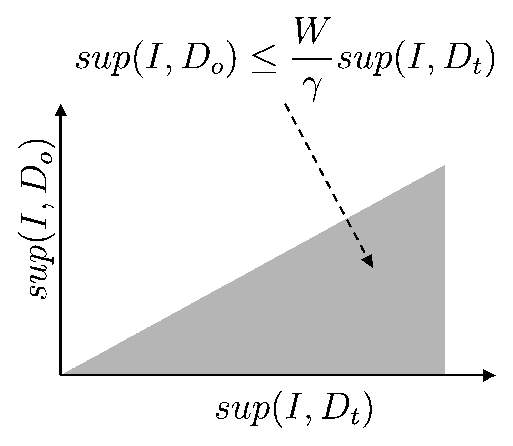
\includegraphics[scale=0.5]{./ep.eps}
\caption{顕在パターン\label{fig:ep}}
\end{center}
\end{minipage}

\begin{minipage}{0.3\hsize}
\begin{center}
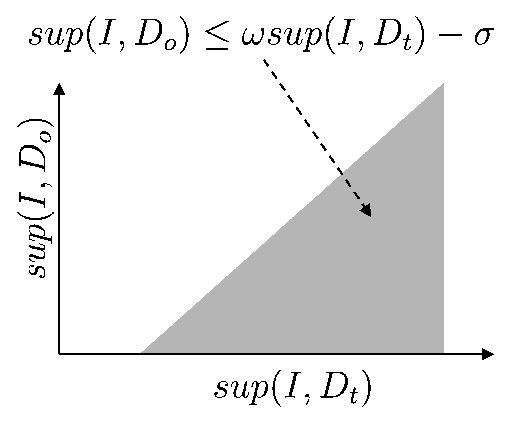
\includegraphics[scale=0.5]{./cp.eps}
\caption{コントラストパターン\label{fig:cp}}
\end{center}
\end{minipage}

\begin{minipage}{0.3\hsize}
\begin{center}
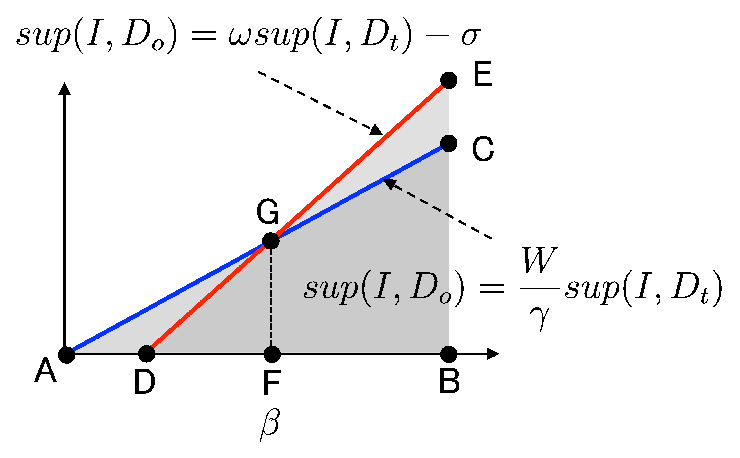
\includegraphics[scale=0.5]{./epcp.eps}
\caption{2つのパターンの関係\label{fig:epcp}}
\end{center}
\end{minipage}


\end{tabular} 
\end{center}
\end{figure} 

LCMでは,ユーザがパラメータ$\omega, \sigma$を与えることで
コントラストパターンを高速に列挙することができる.
コントラストパターンの列挙においては、$sup(I,D_t)$が大きくなればなるほど、
$sup(I,D_o)$との差が相対的に小さいパターンが列挙されることもあり、
そのようなパターンはクラス$c_t$に特徴的なパターンとは言えなくなる。
この欠点を回避するために、本コマンドでは顕在パターンの列挙を採用している。

ここで問題となるのは、コントラストパターンを列挙するLCMを使って、
いかに顕在パターンを列挙するかであり、以下に本コマンドで採用している方法を示す。

図\ref{fig:epcp}は、図\ref{fig:ep}と図\ref{fig:cp}を重ねた図である。
ここでは顕在パターンの領域ABCを全て列挙するのではなく、
$sup(I,D_t)\ge\beta$($\beta$は本コマンドS=で指定するパラメータ)を満たす領域GFCBに属する顕在パターンの列挙を考える。
LCMによって列挙されるパターンは、$\triangle{DEB}$に属するパターンであるが、
直線DEは、$\sigma$と$\omega$を定めることによって決まる。
まず$\sigma$は、直線ACと直線DEの交点Gの$x$座標が、ちょうど$\beta$になるように
設定する(式(\ref{sigma_beta}):$\omega$の決め方は後述)。
そうすることで、LCMが列挙した全パターンから、
$\triangle{DFG}$および$\triangle{EGC}$に属する
パターンを削除すれば、目的とする顕在パターンを列挙することが可能となる。

\begin{equation}
\sigma=\beta (\omega-\frac{W}{\gamma})  \label{sigma_beta}
\end{equation}



次に$\omega$であるが、これは直線DEの傾きを決めることに対応する。
一般的に$\triangle{EGC}$に属するパターンより、$\triangle{DGF}$に属するパターンの方が遥かに多いので、
$\omega$をできる限り大きくする方が効率的である。

しかしながら、$\omega$はトランザクションの重みであり、計算機上で件数をカウント
する変数の型の最大値に制約される。
その最大値を$maxInt$とすると、$\omega sup(I,D_t)\le maxInt$の制約を
満たしていなければならない。
$sup(I,D_t)$は$|D_p|$を超えることはないので、$\omega$を式(\ref{omega})のとおり
指定することで、$\triangle{DFG}$の列挙数を最小化できる。

\begin{equation}
\omega=\frac{maxInt}{|D_t|} \label{omega}
\end{equation}

\begin{thebibliography}{9}
\bibitem{Uno2004}
Takeaki Uno, Tatsuya Asai, Yuzo Uchida, Hiroki Arimura, "An Efficient Algorithm for Enumerating Closed Patterns in Transaction Databases", {\it Discovery Science 2004}, LNAI 3245, pp.16-31.
\bibitem{UnoWeb}
http://research.nii.ac.jp/~uno/codes-j.htm
\end{thebibliography}

\end{document}

